\section{Problem Overview}
One of the things currently unclear with respect to this piece of research is the
specification of the problems, and how we are sending that information to an LLM.
There are two things we think we'll want to do:

\begin{wrapfigure}{l}{8cm}
   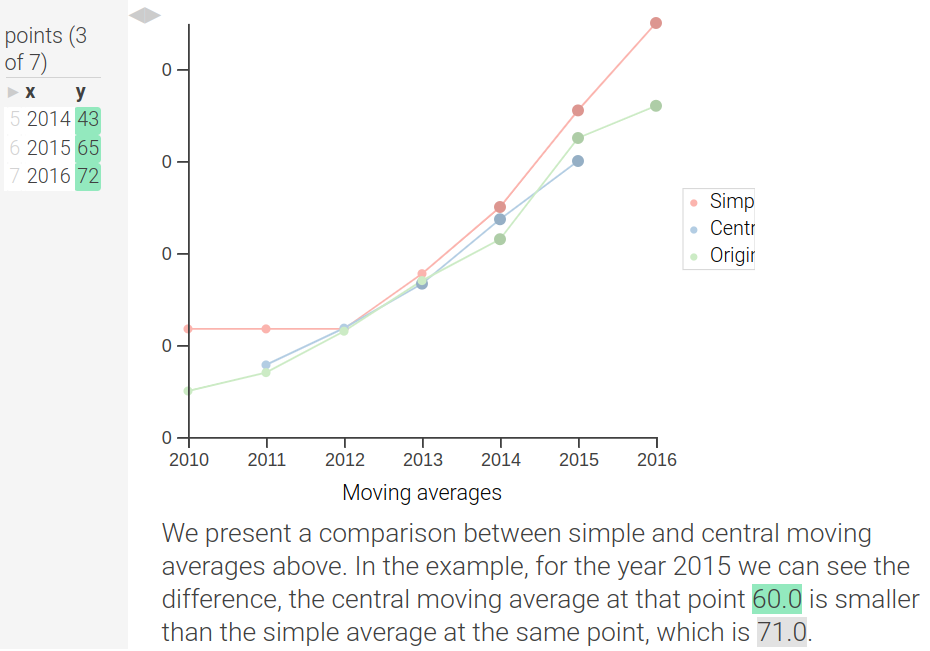
\includegraphics[width=0.5\textwidth]{fig/moving-average example.png}
   \caption{Example of text linking, using moving average example program}
   \label{fig:mavg}
\end{wrapfigure}

\paragraph*{Synthesizing numerical/structural expressions related to data:}
if we are referring to a simple aggregate summary of data, we want to be able
to synthesize an in-place expression that helps out explanation. For example,
if we are explaining a bar-chart: ``the total for the USA, in the year 2015 is
\kw{\{totalFor "USA" data2015\}}''. In many cases, we can write this ourselves,
but would like to be able to synthesize the expression in brackets.
For a real example, consider the image in \figref{mavg}. 

\paragraph*{Synthesizing string expressions based on those numerical expressions:}
this is similar to the nombre library in R, once we are able to synthesize references
to numerical expressions and data, we want to be able to take those, and use them to
create small strings to splice into an explanation. For example ``the \{data for the USA\} is more than \{data for Germany\}''
could be generated by an expression like ``\kw{compare (totalFor "USA" data2015) (compare totalFor "Germany" data2015)}'',
where the function \kw{compare} is itself synthesize by the LLM.
